\documentclass{beamer}
\usepackage{listings}
\lstset{
%language=C,
frame=single, 
breaklines=true,
columns=fullflexible
}
\usepackage{graphicx}
\graphicspath{ {./Images/} }
\usepackage{subcaption}
\usepackage{url}
\usepackage{tikz}
\usepackage{tkz-euclide} % loads  TikZ and tkz-base
%\usetkzobj{all}
\usetikzlibrary{calc,math}
\usepackage{float}
\newcommand\norm[1]{\left\lVert#1\right\rVert}
\renewcommand{\vec}[1]{\mathbf{#1}}
\usepackage[export]{adjustbox}
\usepackage[utf8]{inputenc}
\usepackage{amsmath}
\usetheme{Boadilla}
\title{Error Performance of Information Decoder for SWIPT With Integrated Receiver
}
\subtitle{By Erica Debels\\ Graduate Student Member, IEEE\\ and Marc Moeneclaey\\ Fellow, IEEE
}
\author{Amaan}
\date{EP20BTECH11003}
\institute{Indian Institute of Technology Hyderabad}
\begin{document}
\begin{frame}
    \titlepage
\end{frame}
\begin{frame}{Abbreviations}
    \begin{itemize}
        \item SWIPT - Simultaneous Wireless Information and Power Transfer
        \item EH - Energy Harvester
        \item ID - Information Decoder
        \item QD - Quadratic Detector
        \item ED - Envelope Detector
        \item RX - Separated Receiver
        \item IoT - Internet of Things
        \item IIE-RX - Integrated Information and Energy Receiver 
        \item SISO - Single-Input Single-Output
        \item ASK - Amplitude Shift Keying
        \item BER - Bit Error Rate 
        \item ADC - Analog to Digital Converter
    \end{itemize}
\end{frame}
\begin{frame}
\frametitle{Index}
\tableofcontents
\end{frame}
    \begin{section}{Abstract}
\begin{frame}{Abstract}
    \begin{itemize}
        \item SWIPT can be realized by means of Integrated Receiver, where both the EH and ID operate on rectified received signal.
        \item Researchers investigate the effect of the non-linearity of rectifier on the error performance of the information decoder when transmitting over a Nakagami-m fading channel.
        \item Demonstrated through analysis and simulation, that, the low-noise error performance strongly depends on the small-signal behaviour of the rectifier.
        \item  Approximating the rectifier by a quadratic detector yields accurate bit error rate results, whereas an over-optimistic error performance is obtained when applying the envelope detector approximation.
    \end{itemize}
\end{frame}
\end{section}
\begin{section}{Introduction}
\begin{frame}
\frametitle{Introduction}
\begin{itemize}
    \item SWIPT is a promising technique for powering energy-limited information-processing devices, which are commonly used in the IoT.
    \item Recently, a new type of RX was proposed, namely IIE-RX, which rectifies the incoming signal, and subsequently splits the rectifier output current between the EH and ID circuits.
    \item Authors investigate the error performance of the ID in the IIE-RX, using biased ASK on a SISO Nakagami-m block-fading channel, with the receiver knowing the distorted ASK constellation at the rectifier output.
    \item The main contribution is the derivation of an analytical expression for the BER of the Maximum Likelihood(ML) detector in the low-noise regime.
\end{itemize}
\end{frame}
\end{section}
\begin{section}{SWIPT with Integrated ID and EH Receiver}
\begin{subsection}{Single antenna IIE-RX}
\begin{frame}{SWIPT with Integrated ID and EH Receiver}
  \begin{itemize}
    \item Considering a single-antenna TX sending symbols $a(k)$ from a normalized constellation(i.e, $E[|a(k)|^2]=1$) over a flat Nakagami-m block-fading channel to a single-antenna IIE-RX.
    \item As discussed, the IIE-RX rectifies the input signal and then splits up the output current between ID and EH.
    \end{itemize}

    \begin{figure}[t]
        \centering
         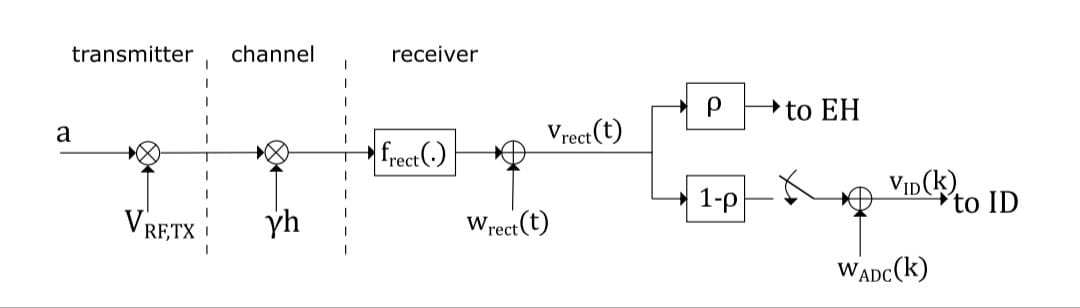
\includegraphics[scale=0.3]{Images/Picture1.jpeg}
        \caption{Block diagram of the Model for the IIE-RX}
        \label{fig:my_label}
        \end{figure}
\end{frame}
\begin{frame}
    Symbols used in the above figure are as described,
    \begin{figure}[t]
        \centering
         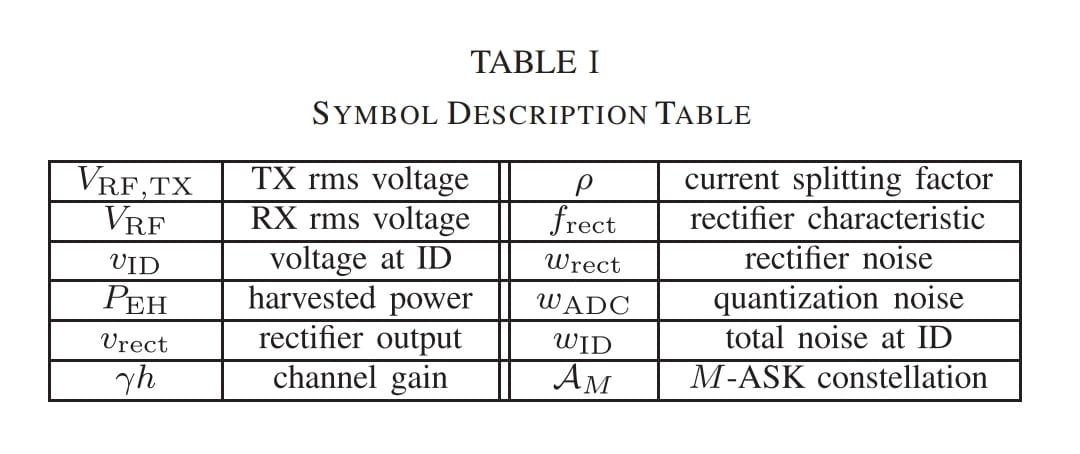
\includegraphics[scale=0.3]{Images/Picture2.jpeg}
        \label{fig:my_label2}
        \end{figure}
\end{frame}
\begin{frame}
    \begin{itemize}
        \item During the $k$th symbol interval ($kT,kT+T$), an RF voltage $v_{RF,TX}(t)$ is applied to the TX antenna, with,
        \begin{align}
            v_{RF,TX}(t)=\sqrt{2}|a(k)|V_{RF,TX}cos(2\pi f_{c}t+\angle a(k))
            \label{eq1}
        \end{align}
      where $|a(k)|$ and $\angle a(k)$ denote the magnitude and phase of $a(k)$; the rms value of $v_{RF,TX}(t)$ in this interval equals $|a(k)|V_{RF,TX}$, making $V_{RF,TX}$ the long-term rms value. 
      \item $\gamma h$ is the channel gain, such that $-20log(\gamma)$ denotes pathloss(in dB) and $h$ is normalized fading gain.
      \item Assuming, $h=|h|e^{j\angle h}$ is constant over a block of $K$ symbol intervals; $|h|$ has a Nakagami-m distribution with $E|h^{2}|=1$ and $\angle h\in[0,2\pi)$, \eqref{eq1} can be written as,
      \begin{align}
          v_{RF,TX}(t)=\sqrt{2}V_{RF}|h||a(k)|cos(2\pi f_{c}t+\theta(k))
          \end{align}
          where, $V_{RF}=\gamma V_{RF,TX}$ and $\theta(k)=\angle a(k)+\angle h$.
      \end{itemize}
\end{frame}
\end{subsection}
\begin{subsection}{Splitting of Rectified Input}

\begin{frame}{}
    \begin{itemize}
        \item The corresponding rectifier output signal $v_rect(t)$ is decomposed as ,
        \begin{align}
            v_{rect}(t)=f_{rect}(|h||a(k)|V_{RF})+w_{rect}(t)
        \end{align}
        \item The function $f_{rect}(A)$ is referred to as the rectifier characteristic, which expresses the rms value A of a sinusoidal input signal.
        \item Considering  the simple rectifier circuit from Fig.,

    \begin{figure}[t]
        \centering
         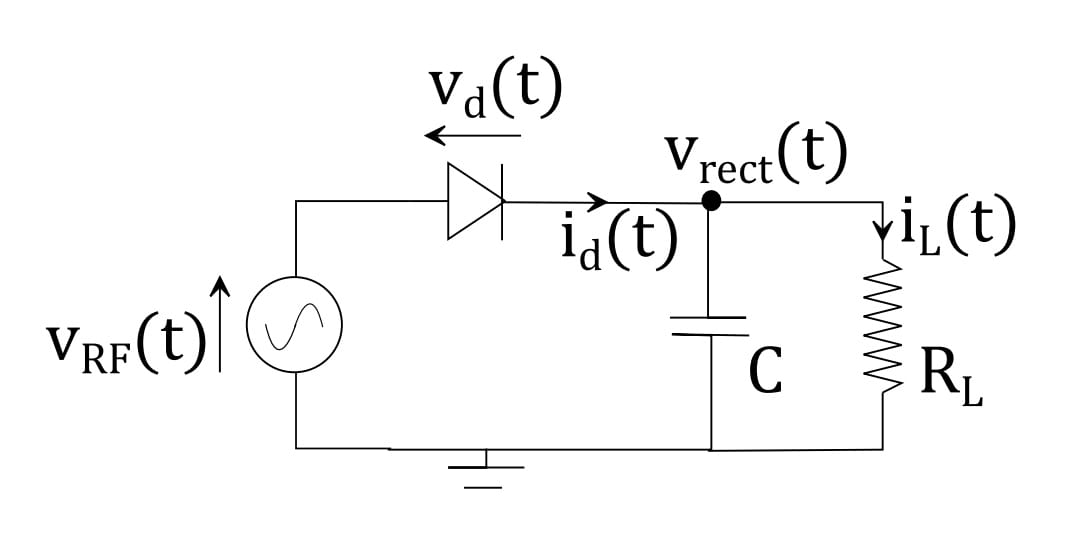
\includegraphics[scale=0.2]{Images/Picture3.jpeg}
         \caption{Simple Rectifier Circuit}
        \label{fig:my_label3}
        \end{figure}
        \end{itemize}
\end{frame}
\begin{frame}
  \begin{itemize}
  
    \item Here,resistive load $R_L$ in Fig. 2 represents the parallel connection of the EH part (load $\frac{R_L}{\rho}$) and the ID part (load $\frac{R_{L}}{1 - \rho }$) of the receiver, which draw currents $\rho \frac{v_{rect}}{R_L}$ and $(1 - \rho ) \frac{v_{rect}}{R_L} $, respectively.
  
        \item The current drawn by the ID part is fed to a sampler and ADC, which results in the voltage $v_{ID}(k)$,
        \begin{align}
            v_{ID}(k)=(1 - \rho )f_{rect}(|h||a(k)|V_{RF})+w_{ID}(k)
            \label{eq3}
        \end{align}
        where, $w_{ID}(k)=(1 - \rho )w_{rect}(kT)+w_{ADC}(k)$, \eqref{eq3} suggests that $v_{ID(k)}$ doesn't depend on the phase of data symbol $a(k)$.
    \end{itemize}
\end{frame}
\end{subsection}
\end{section}
\begin{section}{Rectifier Characteristic}
\begin{frame}{Rectifier Characteristic}
    \begin{itemize}
        \item We determine the characteristic $f_{rect}(A)$ of the rectifier from above fig. by solving the differential equation,
        \begin{align}
            C\frac{dv_{rect}}{dt}+\frac{v_{rect}}{R_L}=I_{s}.(e^{\frac{1}{nv_{th}}}-1)
        \end{align}
        where $V_{th}$ is thermal voltage and the diode is characterized by the reverse saturation current $I_{s}$ and ideality factor $n$. 
        \item On solving using proper assumptions, we get,
        \begin{align}
            f_{rect}(A)=\frac{1}{2}\left(\frac{1}{R_{L}I_{s}}+\frac{1}{nV_{th}}\right)^{-1}.\left(\frac{A}{nV_{th}}\right)^2
        \end{align}
    \end{itemize}
\end{frame}

\begin{frame}
    \begin{figure}[t]
        \centering
         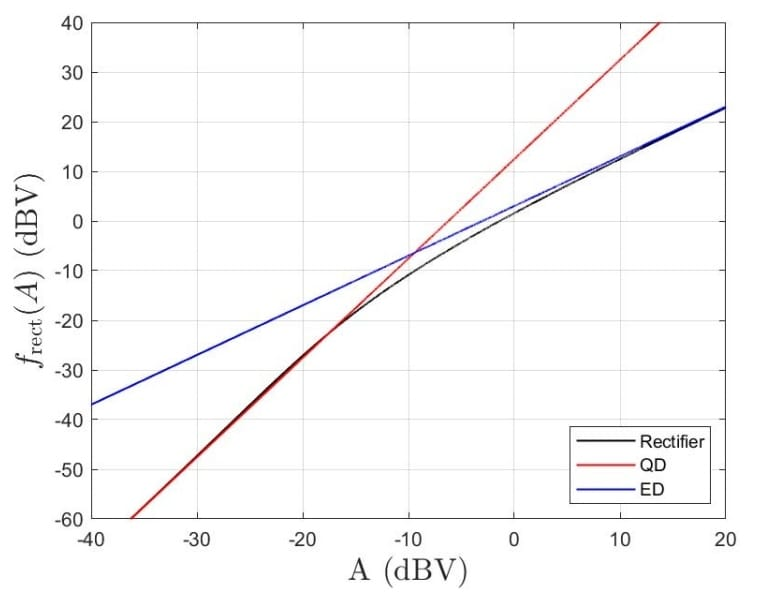
\includegraphics[scale=0.3]{Images/Picture4.jpeg}
         \caption{Rectifier Characteristics showing DC output voltage versus rms input voltage.}
        \label{fig:my_label4}
        \end{figure}
\end{frame}
\end{section}
\begin{section}{BER Analysis}
\begin{frame}{BER Analysis}
\begin{itemize}
    \item Considering the transmission of uncoded symbols from biased $M$-ASK constellation $A_{M}$ .
    \item This constellation gets distorted by the rectifier: the signal component in $v_{ID}(k)$ corresponding to $a(k) =\alpha_{\ell}$ is denoted as,
    \begin{align}
        S_{\ell}=(1 - \rho ) f_{rect}(|h|\alpha_{\ell}V{RF})
    \end{align}
    \item For given $|h|$, the BER is given by,
    \begin{align}
        BER=\frac{1}{Mlog_{2}M}\sum\limits_{i,j=0}^{M-1}n_{i,j}P_{i,j}
    \end{align}
    where $n_{i,j}$ is the number of bits in which $\alpha_{i}$ and $\alpha_{j}$ differ and $P_{i,j}$ is the probability that $\alpha_i$ is detected when $\alpha_j$ is transmitted. 
\end{itemize}
\end{frame}
\begin{frame}
    \begin{itemize}
    \item After performing extensive calculation, it is obtained that,
    \begin{align}
        BER_{avg}=C_{A_{M}}(m,\beta).\left(\frac{\sigma_{ID}^{2/\beta}}{V_{RF}^2}\right)^m
    \label{eq9}
    \end{align}
    where $m$ is the Nakagami parameter, $\beta$ is the variable which tells whether the detector is ED($\beta=1$) or QD($\beta=2$) and,
    \begin{align}
        C_{A_{M}}(m,\beta)=\frac{1}{Mlog_{2}M}.\sum\limits_{i,j=0}^{M-1}n_{i,j}D(m,\beta,i,j)
    \end{align}
    \item From \eqref{eq9}, we can say, for small $\sigma_{ID}$, 
    \begin{align}
        BER_{avg} \propto \left(\frac{\sigma_{ID}^{2/\beta}}{V_{RF}^2}\right)^m
    \end{align}
    this indicates a performance advantage of ED over the rectifier for small $\sigma_{ID}$.
    \end{itemize}
\end{frame}
\begin{frame}
    \begin{figure}[t]
        \centering
         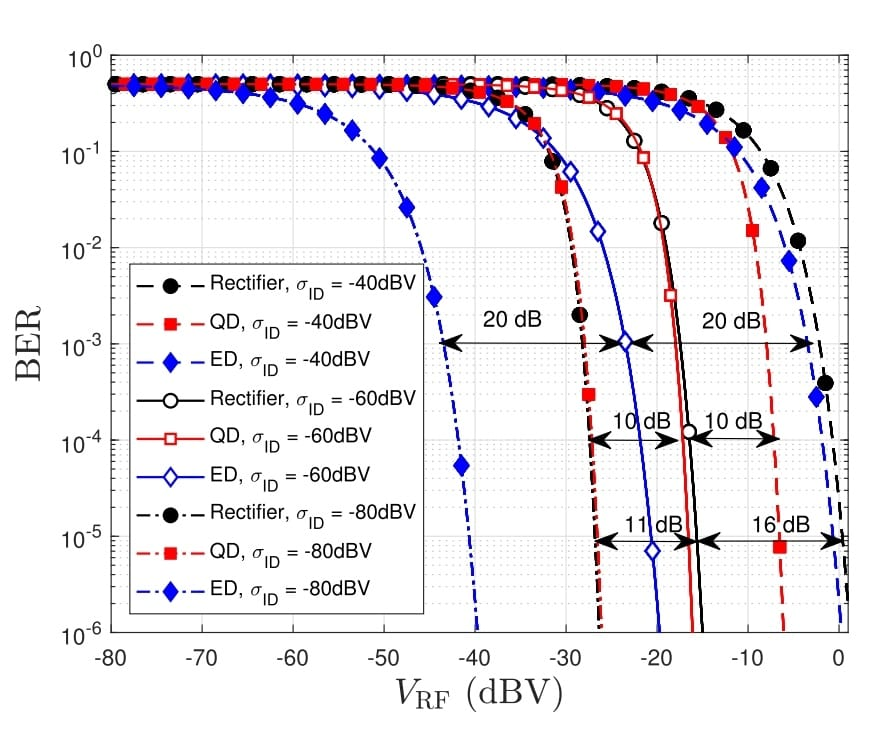
\includegraphics[scale=0.3]{Images/Picture5.jpg}
         \caption{ Conditional BER ($|h| = 1$) versus VRF (2-ASK).}
        \label{fig:my_label5}
        \end{figure}
\end{frame}
\end{section}
\begin{section}{Conclusion}
    \begin{frame}{Conclusion}
    \begin{itemize}
        \item It is investigated the BER of the ID for SWIPT with an IIE-RX, for the uncoded transmission of biased ASK on a Nakagami-m fading channel, and presented an analytical expression for the resulting BER in the small-noise regime.
        \item The characteristics of the rectifier and the QD differ considerably for larger input signals, but their small-noise BER curves nearly coincide.
        \item 
    \end{itemize}
\end{frame}
\end{section}
\begin{frame}
    \centering  \Huge
    \emph{ Thank You}\\
    \vspace{2cm}
    \large
\end{frame}

\end{document}